\thispagestyle{plain}
\newgeometry{margin=2.5cm}
\section{Réalisation de l'application}
\subsection{Création de compte}
La première étape pour utiliser l'application SPN-Cars est de créer un compte. Ce compte permettra aux utilisateurs de bénéficier de tous les services offerts par l'application.\\
\noindent Pour créer un compte l'utilisateur a la possibilité de choisir trois méthodes : Créer un compte avec son émail et choisir un mot de passe, ou créer un compte tout simplement en utilisant l'option de création de compte avec son compte Google ou Apple.
\subsection{Authentification}
L'authentification est la première étape dans le cycle de vie de l'application, lors du premier démarrage de l'application il est nécessaire de vérifier si l'utilisateur est déjà connecté à l'application. Grâce à cette étape on peut identifier l'utilisateur, et limiter les requêtes envoyées au serveur back-end.\\
\noindent Pour s'authentifier l'utilisateur peut choisir trois méthodes différentes : Email et mot de passe, avec son compte Google, ou avec son compte Apple.
\vspace{1cm}
\begin{figure}[H]
    \centering
    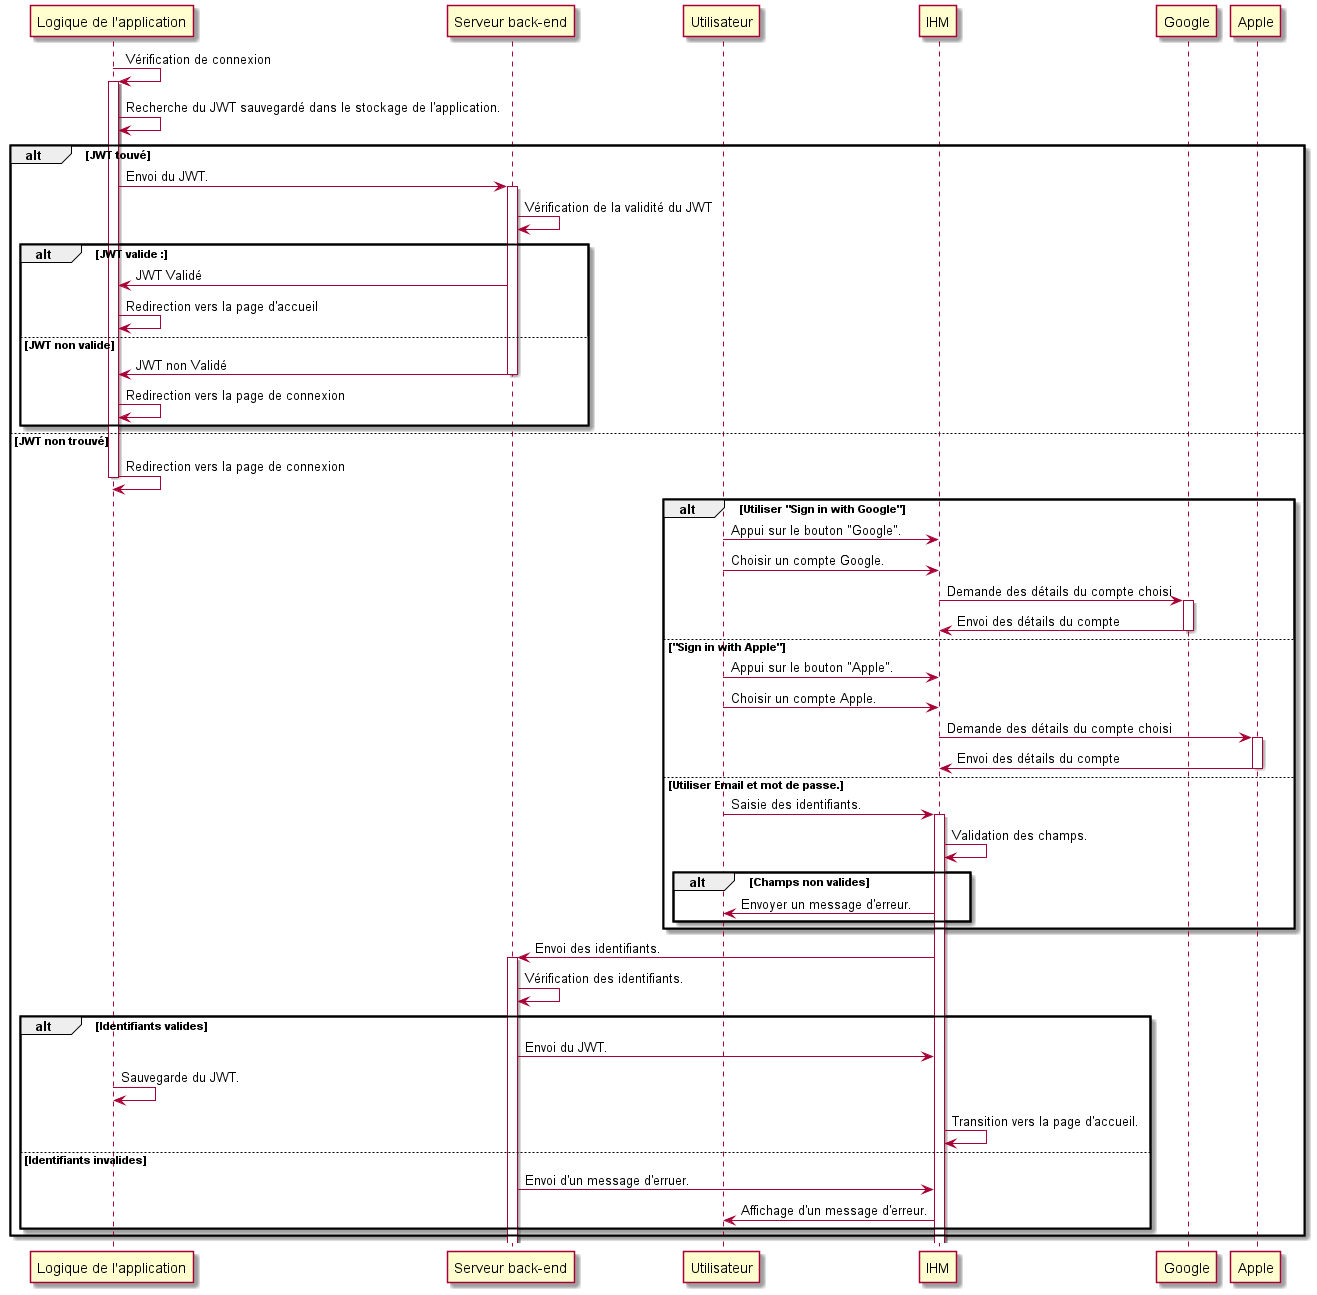
\includegraphics[width = \textwidth]{uml/Authentification.png}
    \vspace{1cm}
    \caption{Diagramme de séquences: Authentification}
    \label{fig:seq_auth}
\end{figure}
\subsection{Page d'accueil}
\subsection{Gestion de profile}
\subsection{Demander un service}
Pour louer une voiture, l'utilisateur a besoin de spécifier tout d'abord les paramètres suivants :
\begin{itemize}
    \item Le type de service demandé (Location / Transfert / Excursion / Long Ride).
    \item L'adresse de départ.
    \item L'heure de départ.
    \item L'adresse d'arrivée (Pas toujours disponible selon le type de service).
    \item L'heure d'arrivée (Pas toujours disponible selon le type de service).
    \item La durée du service demandé (Pas toujours disponible selon le type de service).
\end{itemize}
\vspace{1cm}
\begin{figure}[H]
    \centering
    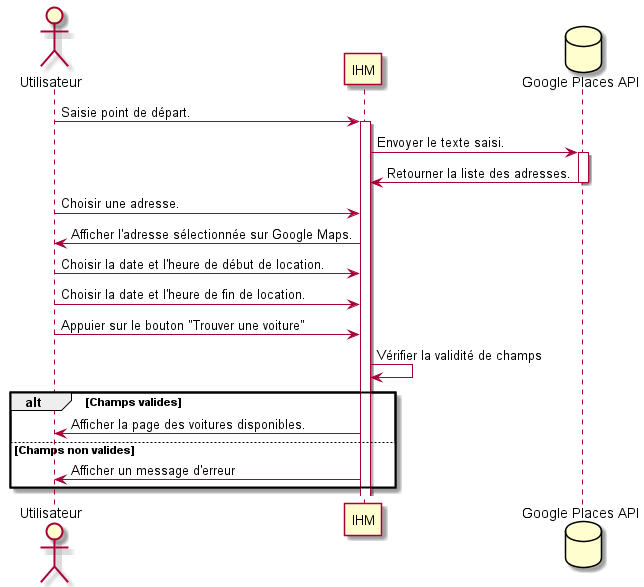
\includegraphics[width = \textwidth]{uml/rent a car.png}
    \vspace{1cm}
    \caption{Diagramme de séquences: Demander une location.}
    \label{fig:seq_location}
\end{figure}
\vspace{1cm}
\begin{figure}[H]
    \centering
    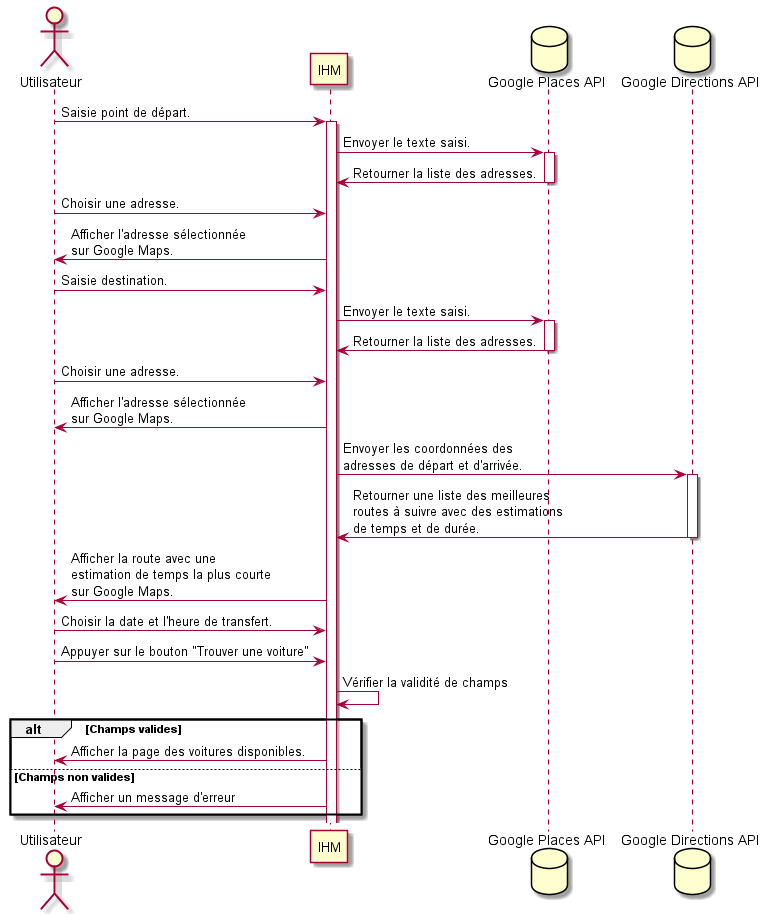
\includegraphics[width = \textwidth]{uml/transfert.png}
    \vspace{1cm}
    \caption{Diagramme de séquences: Demander un transfert.}
    \label{fig:seq_transfert}
\end{figure}
\subsection{Affichage des voitures disponibles}
Après sélection des informations nécessaires par l'utilisateur, une recherche des voitures qui répondent aux critères de recherche choisis. Une fois une liste de voitures est prête, les voitures seront affichés. L'utilisateur peut appuyer sur une voiture pour découvrir ses caractéristiques et choisir ensuite de la louer ou continuer sa recherche.
Le diagramme suivant explique la procédure de la sélection de voitures.
\vspace{1cm}
\begin{figure}[H]
    \centering
    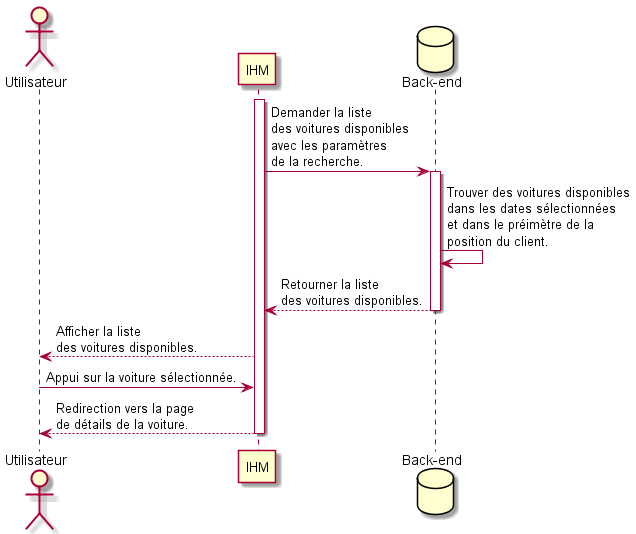
\includegraphics[width = \textwidth]{uml/choisir voiture.png}
    \vspace{1cm}
    \caption{Diagramme de séquences : Choisir une voiture}
    \label{fig:seq_car_select}
\end{figure}
\subsection{Paiement}
\subsection{Localiser une voiture}
\subsection{Messagerie instantanée}